\documentclass[12pt,letterpaper]{article}
\usepackage{fullpage}
\usepackage[top=2cm, bottom=4.5cm, left=2.5cm, right=2.5cm]{geometry}
\usepackage{amsmath,amsthm,amsfonts,amssymb,amscd}
\usepackage{lastpage}
\usepackage{enumerate}
\usepackage{fancyhdr}
\usepackage{mathrsfs}
\usepackage{xcolor}
\usepackage{graphicx}
\usepackage{listings}
\usepackage{hyperref}  
\usepackage{tikz}      
\usepackage{pgf}

\usepackage[scaled=0.85]{FiraMono}

\usetikzlibrary{arrows, automata}

\hypersetup{
    colorlinks=true,
    linkcolor=blue,
    linkbordercolor={0 0 1}
}
 
\newtheorem*{thm}{Theorem}

\renewcommand\lstlistingname{Algorithm}
\renewcommand\lstlistlistingname{Algorithms}
\def\lstlistingautorefname{Alg.}

\lstdefinestyle{Python}{
    language     = Python,
    aboveskip    = 3mm,
    belowskip    = 3mm,
    frame        = lines, 
    basicstyle   = \footnotesize\ttfamily,
    keywordstyle = \color{blue},
    stringstyle  = \color{green},
    commentstyle = \color{red}\small\ttfamily
}

\setlength{\parindent}{0.0in}
\setlength{\parskip}{0.05in}

% Edit these as appropriate
\newcommand\course{CSE 3500}
\newcommand\hwnumber{0}
\newcommand\NetIDa{mfm19005}

\pagestyle{fancyplain}
\headheight 35pt
\lhead{\NetIDa}
\chead{\textbf{\Large Homework \hwnumber}}
\rhead{\course \\ \today}
\lfoot{}
\cfoot{}
\rfoot{\small\thepage}
\headsep 1.5em

\begin{document}

\begin{center}
    \LARGE Problem Set
\end{center}



\section*{Problem 0 -- Collaboration Policy (10\%)}
Read and sign the Collaboration Policy in the Course Content folder on HuskyCT.
Hand in your signed form with your homework submission.
We cannot grade your work without a signed form.

$\hfill \break$
\textit{I have read and signed the form.}

\section*{Problem 1 -- Introductions (10\%)}
The goal of this problem is to introduce yourself to the course staff and to think about what you want to get out of the course.
Write at most two paragraphs about yourself.
This may include your academic and non-academic interests, preferred programming languages, courses that you are excited to take in the future, or areas of computer science that you find the most interesting.
Finish by describing what do you want to learn by taking this course.
Think about what would be most beneficial to your prospective career.

$\hfill \break$
Hello, my name is Mike Medved - I am currently a Junior Computer Science major pursuing a Computational Data Analytics concentration and Information Assurance minor here at UConn. I am really interested in Cyber Security, Cloud-related topics, and am currently a full stack developer. I hope to land a job in one or more of those fields once I graduate, and am currently working on some larger scale projects, such as my website for UConn-related information, \href{https://cobalt.lol}{\textbf{Cobalt}}. My favorite programming language has to be TypeScript, since it is very light but exposes a very powerful types system, and leverages the full might of the npm registry.

$\hfill \break$
I am to improve my knowledge of the more theoretical side of programming, if you can call it that, by learning and better understanding algorithmic design, optimization, and analysis. Not only will this make me a more well-rounded and performance-conscious developer, but it will help out when performing technical interviews at some of the companies I am planning to apply to.

\newpage

\section*{Problem 2 -- Preliminaries (10\%)}
This problem tests your retention of prerequisite materials.
If some of these problems are difficult, please go back and review material from the prerequisites.
\begin{enumerate}
    \item How many permutations are there of the set of $n$ numbers?
    \begin{enumerate}
        \item There are $n!$ permutations - by using the formula for permutations when $k = n$, we can see that $P(n, k) = \frac{n!}{(n-k)!} = n!$
    \end{enumerate}
    \item How many subsets of three numbers are there from a set of $n$ numbers?
    \begin{enumerate}
        \item The number of subsets of three numbers for a set of $n$ numbers is $n^3$. This is because there are $n$ possible choices for the first number, $n$ possible choices for the second number, and $n$ possible choices for the third number.
    \end{enumerate}
    \item How many subsets of $S$ are there when $|S|=n$?
    \begin{enumerate}
        \item There are $2^n$ subsets when $|S|=n$.
    \end{enumerate}
\end{enumerate}

\newpage

\section*{Problem 3 -- Complexity (20\%)}

\begin{enumerate}
    \item For functions $A$ and $B$ and constant $c>1$, indicate which of $\{A = O(B),A = \Omega(B),A = \Theta(B)\}$ holds. Here, we use the notation that $log_2=lg$. \textit{Hint: for these problems it is useful to know some mathematical identities. See CLRS section 3.2 or \textbf{standard\_notations\_and\_common\_functions.pdf} in HuskyCT Lecture 2 course notes.} 
    \begin{enumerate}
        \item $A=n^c$, $B=c^n$
        \begin{itemize}
            \item $A = O(B)$ because $c^n$ will outgrow $n^c$ since $n > c$ with respect to the exponent.
        \end{itemize}
        \item $A=n^{lg(c)}$, $B=c^{lg(n)}$
        \begin{itemize}
            \item $A = \Theta(B)$ because $n^{lg(c)}$ and $c^{lg(n)}$ will be equal when $n = c$.
        \end{itemize}
        \item $A=lg(n!)$, $B=lg(n^n)$
        \begin{itemize}
            \item $A = O(B)$ because $lg(n^n)$ will outgrow $lg(n!)$ since $n^n$ grows faster than $n!$.
        \end{itemize}
        \item $A=3^{3^n}$, $B=3^{n^2}$
        \begin{itemize}
            \item $A = \Omega(B)$ because $3^{3^n}$ will outgrow $3^{n^2}$ since $3^n > n^2$ with respect to the exponent.
        \end{itemize}
    \end{enumerate}
    \vspace{1in}
    \item Place the following functions in increasing order of growth rate. I.e. if $g$ follows $f$ then $f=O(g)$ is true.
    \begin{enumerate}
        \item $n^e$, 
        \item $n^{\lg(n)}$
        \item $n^\pi$, 
        \item $\lg(n!)$
        \item $2^{\sqrt{\lg(n)}}$
        \item $n$
    \end{enumerate}

    $$
        2^{\sqrt{\lg(n)}} < n < lg(n!) < n^e < n^{\lg(n)} < n^\pi
    $$
\end{enumerate}

\newpage

\section*{Problem 4 --  Vinder (30\%)}
Vinder is a new smartphone app designed to make it easier for everyone to eat their vegetables. 
Vinder compares your genetic information with a large database of vegetable genetic sequences to match you with the right vegetable based on sequence similarity. 
Specifically, it computes the longest common subsequence between your DNA sequence and the DNA sequences of thousands of vegetables. 

An $n$-length \textit{DNA sequence}, $A$, is an ordered collection of elements $\in [A,C,G,T]$, or $A\in[A,C,G,T]^n$.
A \textit{subsequence} is a sequence formed by deleting elements from another sequence, thus preserving the original order.
A $k$-length \textit{prefix} of sequence $A$ is the first $k$ elements of $A$.
For example, $A=[A,C,C,G,G,A,A,T,C]$ is a sequence. $[A,C,A,T]$ and $[C]$ are subsequences of $A$ but $[T,A]$ is not. $[A,C,C,G]$ is a $4$-prefix of $A$ and $[ ]$ is the $0$-prefix.

Our goal is to find the longest common subsequence (LCS) of $A$, the human DNA sequence, and sequences $B^k \in D$ where $D$ is the database of vegetable DNA sequences and $k=1,...,|D|$.
This solution can be found efficiently using dynamic programming. 
At a high-level, the algorithm is:
\begin{enumerate}
    \item For each sequence $B^k\in D$
    \item Initialize the length of the LCS to $0$.
    \item Let $A_i$ denote the $i^{th}$ element of $A$. 
    Consider each pair of $A_i$ and $B^k_j$; either $A_i=B^k_j$ or $A_i \neq B^k_j$.
    \begin{itemize}
        \item If $A_i=B^k_j$, then the length of the LCS of the $i$-prefix of $A$ and $j$-prefix of $B^k$ is one more than the LCS of the $i-1$-prefix of $A$ and $j-1$-prefix of $B^k$.
        \item If $A_i \neq B^k_j$, then we cannot extend the LCS. 
        Instead, we conclude that the LCS up to $(A_i,B^k_j)$ is the maximum of the LCS up to $(A_{i-1},B^k_j)$ or $(A_i,B^k_{j-1})$.
    \end{itemize}
\end{enumerate}
The two aforementioned cases sum up the possibilities at $(A_i,B^k_j)$.
We can use these to recursively define the LCS in terms of smaller problem solutions.
Your goal is to describe the algorithm to do this.
\newpage
\begin{enumerate}
    \item Describe an algorithm to find the length of the LCS that does not use dynamic programming. 
    You do not have to write pseudocode, simply describe the algorithm in enough detail so that we understand it. 
    What is the runtime?
    Why is it correct?
    You may keep your answers informal. 
    
    \lstset{caption={Naive Approach for Longest Common Subsequence}}
     \begin{lstlisting}[style = Python]
def lcs(a, b):
    result = 0
    for i in range(len(a)):
        for j in range(len(b)):
            if a[i] == b[j]:
                result = max(result, 1 + lcs(a[i+1:], b[j+1:]))
                
    return result
    \end{lstlisting}

    The runtime of this naive approach is $O(n^2)$ since we traverse the two strings, in their entirety, twice using the double for-loop setup seen above.

    This approach is correct, in that it returns the correct result for any two given inputs. However, it can be improved by using memoization and dynamic programming in order to reduce the amount of recalculations necessary, which in turn will improve both the time and space complexities.

    \vspace{0.25in}
    
    \item Write out the recurrence relation used in the algorithm defined in the problems description (not part 1 of the answers). 
    That is, write out how the LCS length can be expressed in terms of smaller instances of the problem.
    
    \begin{equation}
        LCS(i,j) = max
        \left\{
            \begin{array}{lr}
                0 & \text{if } i=0 \text{ or } j=0\\
                1+LCS(a_{i-1}, b_{j-1}) & \text{if } A_i = B_j^k\\
                LCS(a_{i-1}, b_j) & \text{if } A_i \neq B_j^k\\
                LCS(a_i, b_{j-1})
            \end{array}
        \right\}
    \end{equation}

    \vspace{0.25in}
    \item Think about how to convert this into a dynamic program. What size table would you need for the LCS problem?
        
    $\hfill \break$
    You would need an $i*j$ dimension table in order to store the maximum LCS of each $A_i \forall B^k \in D$.

    \vspace{0.25in}

    \newpage
    \item Interpret each table entry. That is, give your explanation for what each entry in the dynamic programming table represents. 
    We discussed how to interpret the entries of the dynamic programming table for the similar problem of \textit{edit distance}.

    $\hfill \break$
    Each $table[i, j]$ represents the maximum LCS result for the intersection of the current $i$-prefix of $A$ and $j$-prefix of $B^k$.
    
    \vspace{0.25in}

    \item Write out the table for $Derek$ and $Asparagus$, where $Derek = [A,C,A,G,G,T,T,A,C]$, and $Asparagus = [T,C,G,G,A,A,T,A,A]$.
    
    \begin{table}[!htb]
        \centering
        \begin{tabular}{lllllllllll}
                                        &                        & \textbf{A}             & \textbf{C}             & \textbf{A}             & \textbf{G}             & \textbf{G}             & \textbf{T}             & \textbf{T}             & \textbf{A}             & \textbf{C}             \\ \cline{2-11} 
        \multicolumn{1}{l|}{}           & \multicolumn{1}{l|}{0} & \multicolumn{1}{l|}{0} & \multicolumn{1}{l|}{0} & \multicolumn{1}{l|}{0} & \multicolumn{1}{l|}{0} & \multicolumn{1}{l|}{0} & \multicolumn{1}{l|}{0} & \multicolumn{1}{l|}{0} & \multicolumn{1}{l|}{0} & \multicolumn{1}{l|}{0} \\ \cline{2-11} 
        \multicolumn{1}{l|}{\textbf{T}} & \multicolumn{1}{l|}{0} & \multicolumn{1}{l|}{0} & \multicolumn{1}{l|}{0} & \multicolumn{1}{l|}{0} & \multicolumn{1}{l|}{0} & \multicolumn{1}{l|}{0} & \multicolumn{1}{l|}{1} & \multicolumn{1}{l|}{1} & \multicolumn{1}{l|}{1} & \multicolumn{1}{l|}{1} \\ \cline{2-11} 
        \multicolumn{1}{l|}{\textbf{C}} & \multicolumn{1}{l|}{0} & \multicolumn{1}{l|}{0} & \multicolumn{1}{l|}{1} & \multicolumn{1}{l|}{1} & \multicolumn{1}{l|}{1} & \multicolumn{1}{l|}{1} & \multicolumn{1}{l|}{1} & \multicolumn{1}{l|}{1} & \multicolumn{1}{l|}{1} & \multicolumn{1}{l|}{2} \\ \cline{2-11} 
        \multicolumn{1}{l|}{\textbf{G}} & \multicolumn{1}{l|}{0} & \multicolumn{1}{l|}{0} & \multicolumn{1}{l|}{1} & \multicolumn{1}{l|}{1} & \multicolumn{1}{l|}{2} & \multicolumn{1}{l|}{2} & \multicolumn{1}{l|}{2} & \multicolumn{1}{l|}{2} & \multicolumn{1}{l|}{2} & \multicolumn{1}{l|}{2} \\ \cline{2-11} 
        \multicolumn{1}{l|}{\textbf{G}} & \multicolumn{1}{l|}{0} & \multicolumn{1}{l|}{0} & \multicolumn{1}{l|}{1} & \multicolumn{1}{l|}{1} & \multicolumn{1}{l|}{2} & \multicolumn{1}{l|}{3} & \multicolumn{1}{l|}{3} & \multicolumn{1}{l|}{3} & \multicolumn{1}{l|}{3} & \multicolumn{1}{l|}{3} \\ \cline{2-11} 
        \multicolumn{1}{l|}{\textbf{A}} & \multicolumn{1}{l|}{0} & \multicolumn{1}{l|}{1} & \multicolumn{1}{l|}{1} & \multicolumn{1}{l|}{2} & \multicolumn{1}{l|}{2} & \multicolumn{1}{l|}{3} & \multicolumn{1}{l|}{3} & \multicolumn{1}{l|}{3} & \multicolumn{1}{l|}{4} & \multicolumn{1}{l|}{4} \\ \cline{2-11} 
        \multicolumn{1}{l|}{\textbf{A}} & \multicolumn{1}{l|}{0} & \multicolumn{1}{l|}{1} & \multicolumn{1}{l|}{1} & \multicolumn{1}{l|}{2} & \multicolumn{1}{l|}{2} & \multicolumn{1}{l|}{3} & \multicolumn{1}{l|}{3} & \multicolumn{1}{l|}{3} & \multicolumn{1}{l|}{4} & \multicolumn{1}{l|}{4} \\ \cline{2-11} 
        \multicolumn{1}{l|}{\textbf{T}} & \multicolumn{1}{l|}{0} & \multicolumn{1}{l|}{1} & \multicolumn{1}{l|}{1} & \multicolumn{1}{l|}{2} & \multicolumn{1}{l|}{2} & \multicolumn{1}{l|}{3} & \multicolumn{1}{l|}{4} & \multicolumn{1}{l|}{4} & \multicolumn{1}{l|}{4} & \multicolumn{1}{l|}{4} \\ \cline{2-11} 
        \multicolumn{1}{l|}{\textbf{A}} & \multicolumn{1}{l|}{0} & \multicolumn{1}{l|}{1} & \multicolumn{1}{l|}{1} & \multicolumn{1}{l|}{2} & \multicolumn{1}{l|}{2} & \multicolumn{1}{l|}{3} & \multicolumn{1}{l|}{4} & \multicolumn{1}{l|}{4} & \multicolumn{1}{l|}{5} & \multicolumn{1}{l|}{5} \\ \cline{2-11} 
        \multicolumn{1}{l|}{\textbf{A}} & \multicolumn{1}{l|}{0} & \multicolumn{1}{l|}{1} & \multicolumn{1}{l|}{1} & \multicolumn{1}{l|}{2} & \multicolumn{1}{l|}{2} & \multicolumn{1}{l|}{3} & \multicolumn{1}{l|}{4} & \multicolumn{1}{l|}{4} & \multicolumn{1}{l|}{5} & \multicolumn{1}{l|}{5} \\ \cline{2-11} 
                                        &                        &                        &                        &                        &                        &                        &                        &                        &                        &                       
        \end{tabular}
    \end{table}

    \newpage

    \item Prove your LCS algorithm's (that you defined in 2-5) correctness. 
    \begin{thm}
        The devised algorithm to calculate LCS(i, j) is correct.
    \end{thm}

    \begin{proof}
        We will prove by induction on $i, j$, traversed in row-major order, that $C[i, j]$ computes the longest common subsequence between the \textit{i-prefix} of A, and \textit{j-prefix} of B, which are supplied as two arbitrary strings to our algorithm.  

        $\hfill \break$
        The longest common subsequence between any string $A$ and a \textit{0-prefix} must be 0, as there are no common characters between an arbitrary string input, and an empty string. This is the base case of our algorithm. We will assume that the algorithm correctly computes the base case by checking the lengths of $A$ and $B$ to see if either are 0 before beginning.
        
        $\hfill \break$
        We will consider arbitrary inputs $A$ and $B$ of length $m$ and $n$ respectively, and integers $i$ and $j$ that are each less than their counterpart, $m$ and $n$ respectively. Consider a strategy $S$ to approach the problem of finding the longest common subsequence between $A$ and $B$. We will assume that $S$ is optimal, and that it returns the correct output. 
        
        $\hfill \break$
        With this strategy $S$, we will consider the final operation conducted by $S$ according to the following rules:

        \begin{enumerate}
            \item If $A[i] = B[j]$, then $S$ will increment the resultant LCS value stored in the table by one.
            \item If $A[i] \neq B[j]$, then we will compute the maximum value of recursing down each function individually, for example we will recurse $LCS(A_{i-1}, B_j)$ and $LCS(A_i, B_{j-1})$ simultaneously, and return the maximum value.
            \item If $A || B == 0$, then $S$ will return 0.
        \end{enumerate}
        
        By our induction hypothesis, $C[i - 1, j - 1]$ computes this value, and thus the expression
        $$1 + LCS(A[i], B[j])$$
        accurately models the result that the optimal strategy $S$ will yield for this case.
        
        $\hfill \break$
        In this way, one of the three options in our three-way \textit{max} function will result in the longest common subsequence our optimal strategy $S$ is looking to yield. Additionally, the options of the 3-way max are intended to cover all potential cases in order to ensure $S$ holds true, and consequently returns a valid and correct result.

        $\hfill \break$
        $\therefore$ The our algorithm will return the correct longest common subsequence for any two arbitrary inputs.
    \end{proof}
    
\end{enumerate}

\newpage
\newpage


\section*{Problem 5 -- Longest Path Problem (20\%)}
We are given a directed, unweighted graph $G=(V,E)$ where $v_i \in V$ for $i=1,...,n$.
Additionally, $G$ is ordered, meaning
\begin{itemize}
    \item An edge can only originate from a vertex with lower index than its destination. Formally, edges may only have the form $(v_i,v_j)$ where $i<j$.
    \item The only \textit{absorbing} node is $v_n$. Absorbing nodes have out-degree $0$.
\end{itemize}

Given an ordered, unweighted, directed graph $G(V,E)$, the \textit{longest path problem} is to compute the longest path length from $v_1$ to $v_n$.

    \lstset{caption={Longest path algorithm}}
    \lstset{label={lst:alg1}}
     \begin{lstlisting}[style = Python]
    def longestPath(v1):
        iter = v1
        length = 0
        while iter.hasOutgoingEdge():
            iter = iter.getEdgeSmallestIndex()
            length += 1
        return length
    \end{lstlisting}

\begin{enumerate}
    \item Demonstrate that Alg. \ref{lst:alg1} does not correctly solve the problem by giving a counter-example as a graph. 
    The function \texttt{iter.hasOutgoingEdge()} returns a boolean indicating whether or not the vertex \texttt{iter} has an outgoing edge.
    The function \\
    \texttt{iter.getEdgeSmallestIndex()} returns the smallest index of all vertices incident from \texttt{iter}. 
    That is, $min_j \{ (iter,v_j) \in E \}$.
    We prefer that your solution be a graph embedding either by hand-drawing and scanning or taking a picture, or drawing it digitally. 
    If none of these options are available, you can simply list the set of edges in the graph.

    \begin{center}
        \scalebox{0.15}{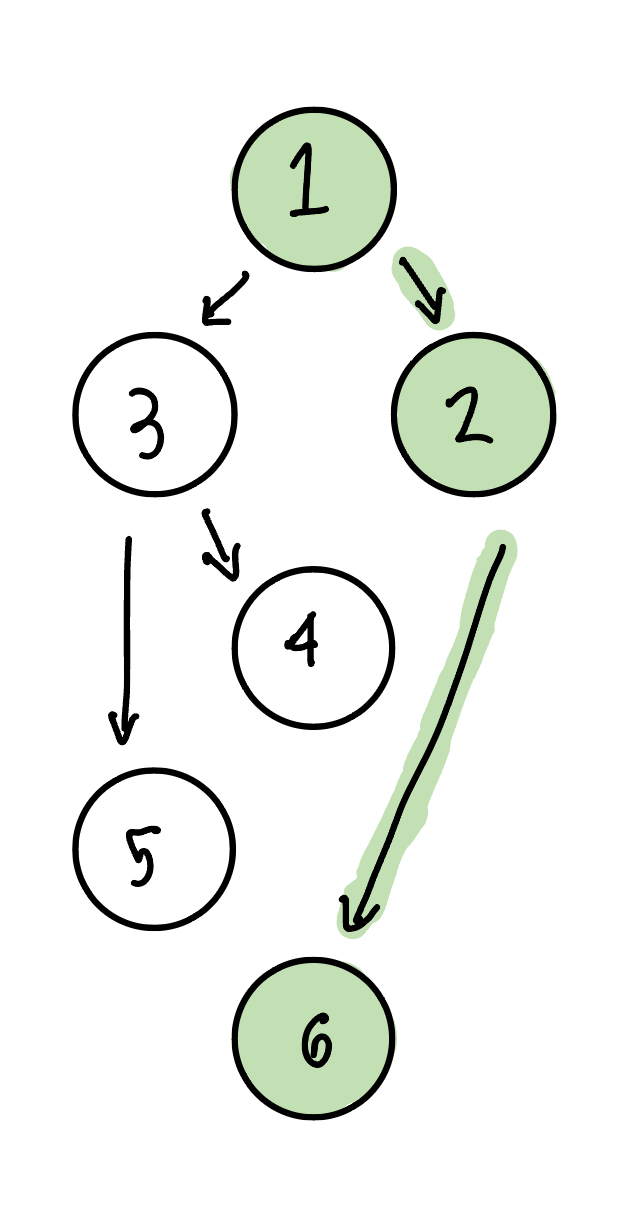
\includegraphics{graph.jpeg}}
    \end{center}

    \newpage

    \item Develop an $O(n^2)$ algorithm for solving the  \textit{longest path problem} in ordered, unweighted, directed graphs. 
    Besides the functions defined above, you are free to use any function associated with graph data structure implementations.

    \lstset{caption={Finding longest path through graph in $O(n^2)$}}
    \begin{lstlisting}[style = Python]
class Graph:
    def init(self, n):
        self.n = n
        self.edges = []
        self.visited = [False] * n

def getLongestPath(self):
    longest = 0
    for i in range(self.n):
        self.visited = [False] * self.n
        longest = max(longest, self.recurse(i, 0))
    return longest

def recurse(self, node, length):
    self.visited[node] = True
    longest = length
    for u, v in self.edges:
        if u == node and not self.visited[v]:
            longest = max(longest, self.recurse(v, length + 1))
    self.visited[node] = False
    return longest
    \end{lstlisting}

\end{enumerate}
\end{document}
